%
% \section{Examples}\label{examples}
%
% This section presents some sample documents. 
%
%
%    The figures are from processed versions of the files. Having latexed
% a file I used DVIPS to get Encapsulated PostScript, then the epstopdf
% script to get a PDF version as well, for example: \\
% \begin{verbatim}
% > latex villon
% > latex villon
% > latex villon
% > dvips -E -o villon.eps villon  % produces villon.eps
% > epstopdf villon.eps            % produces villon.pdf
% \end{verbatim}
%
% For a multipage example, DVIPS has an option to output a range of pages (-p
% for the first and -l (letter l) for the last).
% For instance, to output a single page, say page 2:\\
% \begin{verbatim}
% > latex djd17nov
% > latex djd17nov
% > latex djd17nov
% > dvips -E -p2 -l2 -o djd17novL.eps djd17nov  % produces djd17novL.eps
% > epstopdf djd17novL.eps                      % produces djd17novL.pdf
% \end{verbatim}
%
%      For those who aren't fascinated by LaTeX code, I show the all the
% typeset results first, then the code that produced them. 
% 
%
% \cleardoublepage
%
% \begin{figure}[p]
% \centering
% 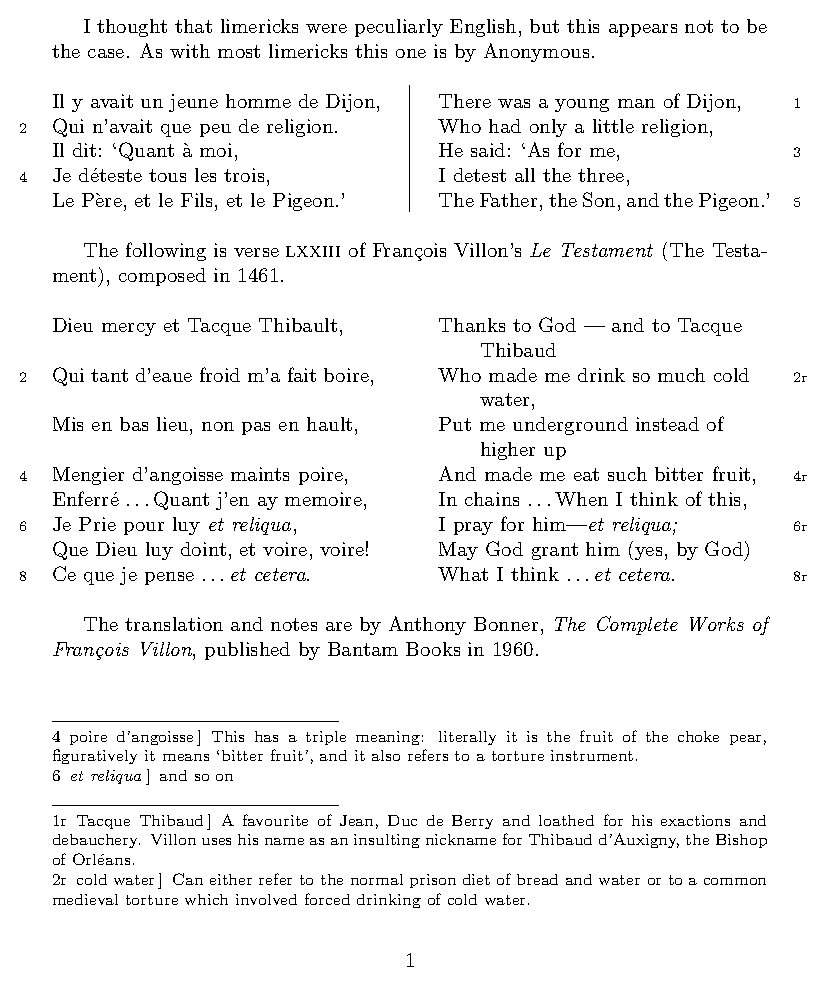
\includegraphics{villon}
% \caption{Output from \file{villon.tex}.}
% \label{villon-out}
% \end{figure}
%
% \begin{figure}[p]
% \centering
% 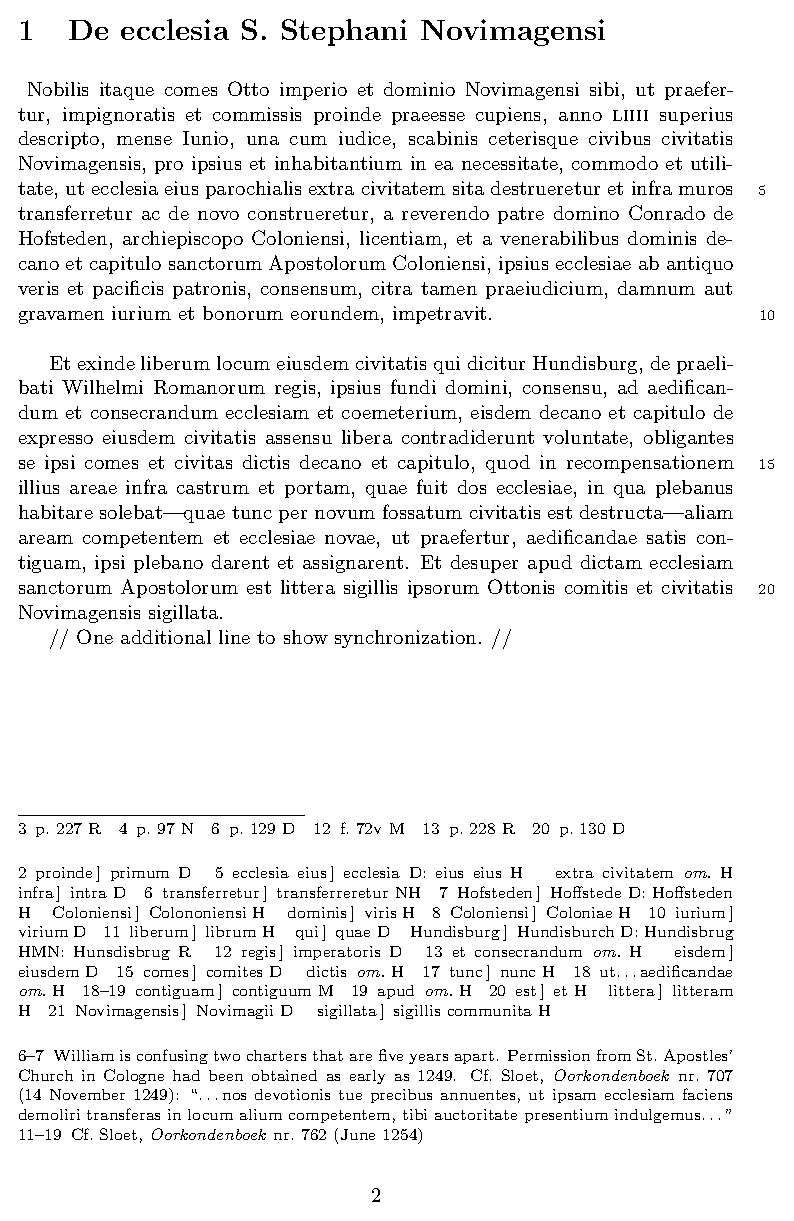
\includegraphics{djd17novL}
% \caption{Left page output from \file{djd17nov.tex}.}
% \label{djdL-out}
% \end{figure}
%
% \begin{figure}[p]
% \centering
% 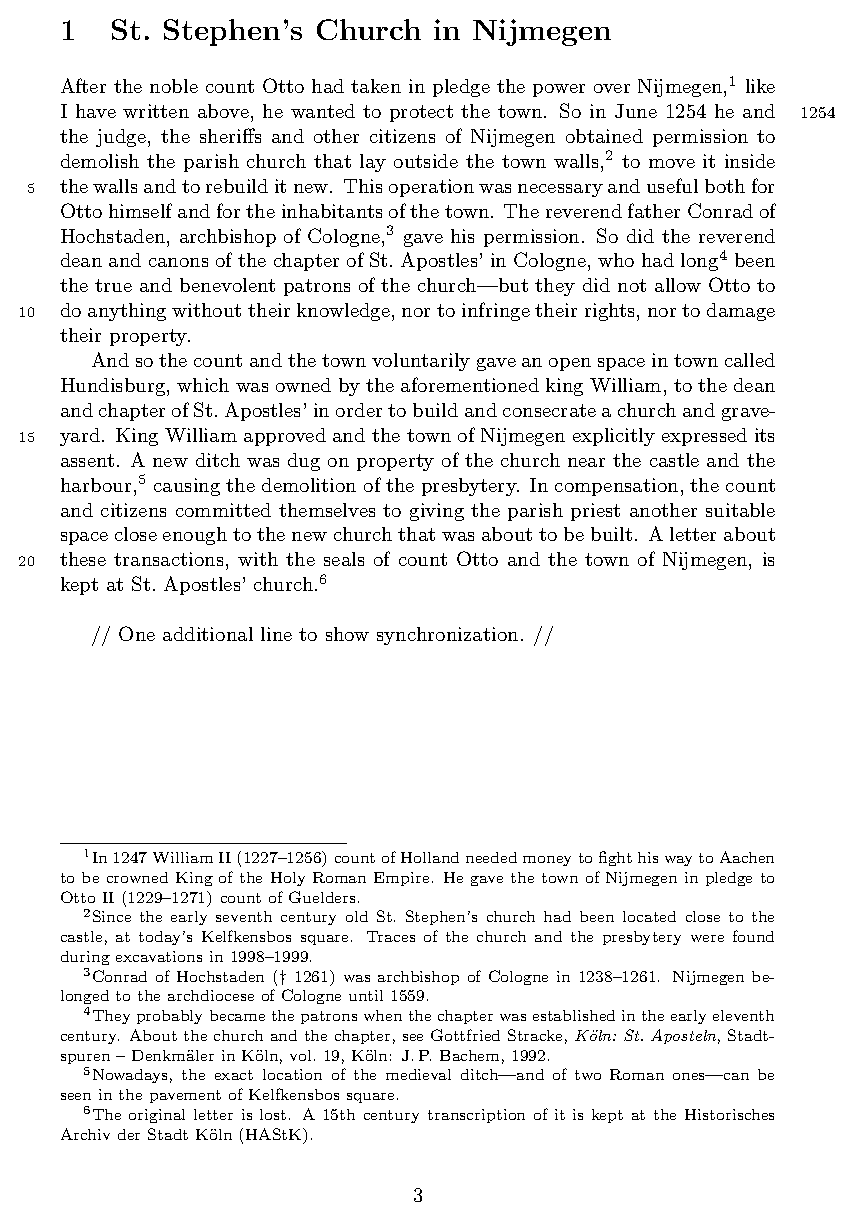
\includegraphics{djd17novR}
% \caption{Right page output from \file{djd17nov.tex}.}
% \label{djdR-out}
% \end{figure}
%
% \begin{figure}[p]
% \centering
% 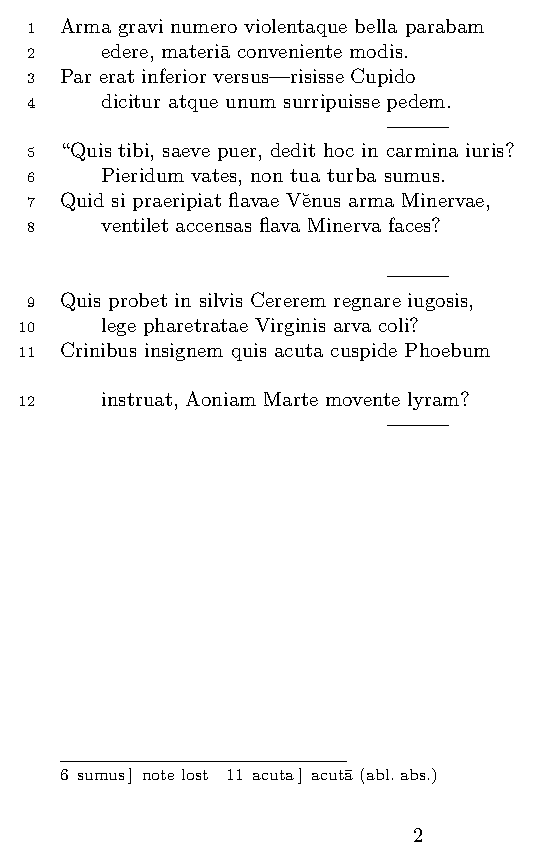
\includegraphics{djdpoems1}
% \caption{First left page output from \file{djdpoems.tex}.}
% \label{djdp1-out}
% \end{figure}
%
% \begin{figure}[p]
% \centering
% 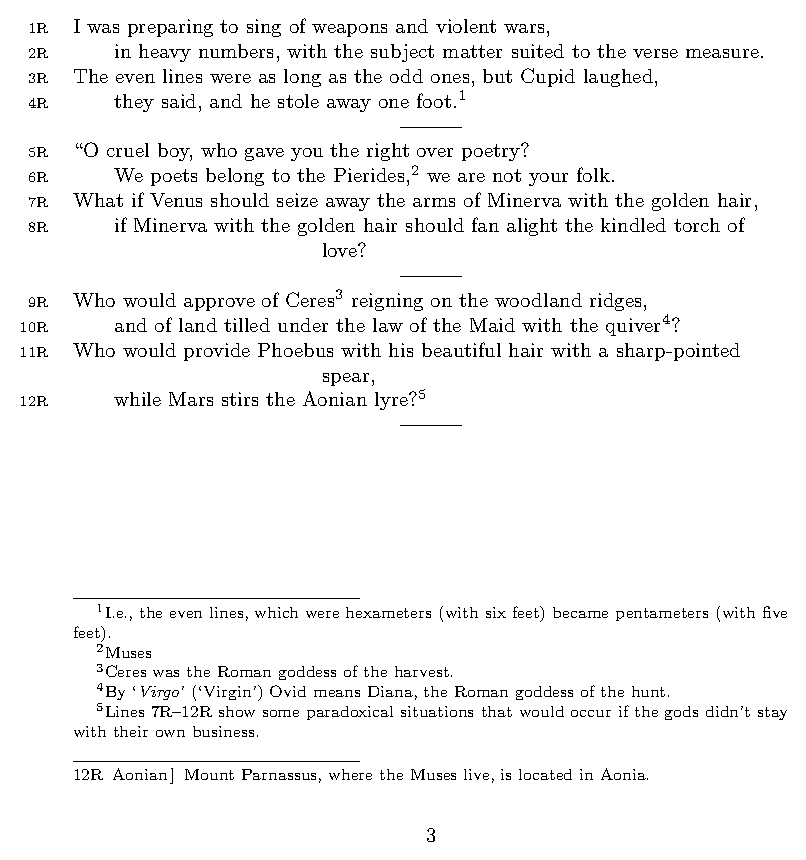
\includegraphics{djdpoems2}
% \caption{First right page output from \file{djdpoems.tex}.}
% \label{djdp2-out}
% \end{figure}
%
% \begin{figure}[p]
% \centering
% 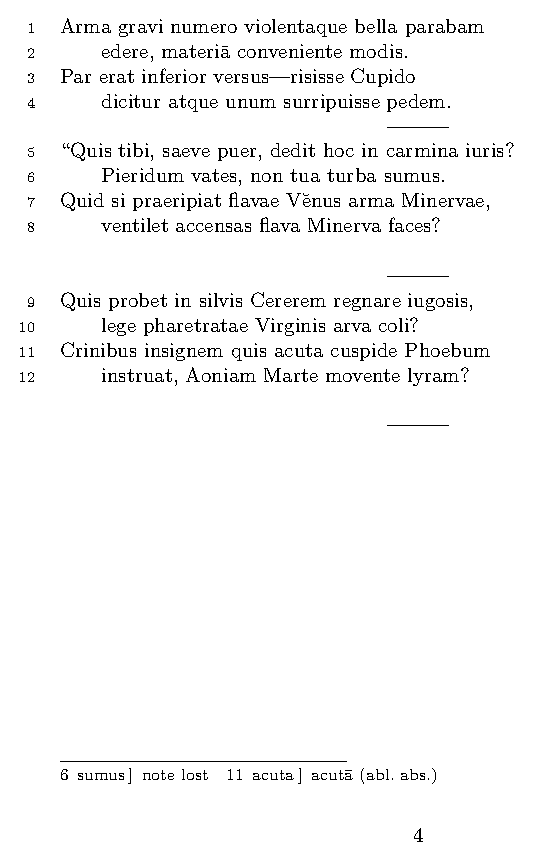
\includegraphics{djdpoems3}
% \caption{Second left page output from \file{djdpoems.tex}.}
% \label{djdp3-out}
% \end{figure}
%
% \begin{figure}[p]
% \centering
% 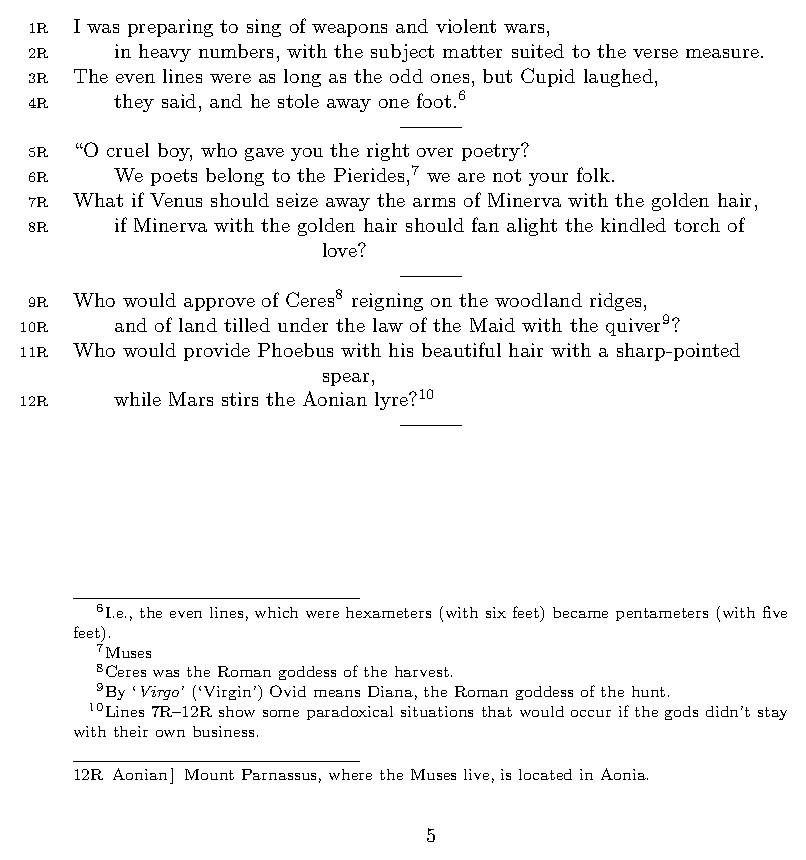
\includegraphics{djdpoems4}
% \caption{Second right page output from \file{djdpoems.tex}.}
% \label{djdp4-out}
% \end{figure}
%
%
%
% \clearpage
%
% \subsection{Parallel column example}\label{example:villon}
%
% This made-up example, \file{villon.tex}, is included to show 
% parallel columns and how they can be interspersed in regular text.
% The verses are set using the \cs{stanza} construct, where each 
% verse line is a chunk.
% The code is given below and the result is shown in Figure~\ref{villon-out}.
%
% \medskip
% \hrule
% \medskip
%    \begin{macrocode}
%<*villon>
%%% villon.tex Example parallel columns
\documentclass{article}
\addtolength{\textheight}{-10\baselineskip}
\usepackage{ledmac,ledpar}
%% Use r instead of R to flag right text line numbers
\renewcommand{\Rlineflag}{r}
%% Use the flag in the notes
\let\oldBfootfmt\Bfootfmt
\renewcommand{\Bfootfmt}[3]{%
  \let\printlines\printlinesR
  \oldBfootfmt{#1}{#2}{#3}}
\begin{document}

I thought that limericks were peculiarly English, but this appears not
to be the case. As with most limericks this one is by Anonymous.

\vspace*{\baselineskip}

\begin{pairs}
%% no indentation
\setstanzaindents{0,0,0,0,0,0,0,0,0}
%% no number flag
\renewcommand{\Rlineflag}{}
%% draw a rule and widen the columns
\setlength{\columnrulewidth}{0.4pt}
\setlength{\Lcolwidth}{0.46\textwidth}
\setlength{\Rcolwidth}{\Lcolwidth}

\begin{Leftside}
%% set left text line numbering sequence
\firstlinenum{2}
\linenumincrement{2}
\linenummargin{left}
\beginnumbering
\stanza
Il y avait un jeune homme de Dijon, &
Qui n'avait que peu de religion. &
Il dit: `Quant \`{a} moi, &
Je d\'{e}teste tous les trois, &
Le P\`{e}re, et le Fils, et le Pigeon.' \&
\endnumbering
\end{Leftside}

\begin{Rightside}
%% different right text line numbering sequence
\firstlinenum{1}
\linenumincrement{2}
\linenummargin{right}
\beginnumbering
\stanza
There was a young man of Dijon, &
Who had only a little religion, &
He said: `As for me, & 
I detest all the three, &
The Father, the Son, and the Pigeon.' \&
\endnumbering
\end{Rightside}

\Columns
\end{pairs}

\vspace*{\baselineskip}

    The following is verse \textsc{lxxiii} of Fran\c{c}ois Villon's 
\textit{Le Testament} (The Testament), composed in 1461.

%% Allow for hanging indentation for long lines
\setstanzaindents{1,0,0,0,0,0,0,0,0}
%% Columns wider than the default
\setlength{\Lcolwidth}{0.46\textwidth}
\setlength{\Rcolwidth}{\Lcolwidth}
\vspace*{\baselineskip}

\begin{pairs}
\begin{Leftside}
\firstlinenum{2}
\linenumincrement{2}
\linenummargin{left}
\beginnumbering
\stanza
Dieu mercy et Tacque Thibault, &
Qui tant d'eaue froid m'a fait boire, &
Mis en bas lieu, non pas en hault, &
Mengier d'angoisse maints \edtext{poire}{\lemma{poire d'angoisse}%
  \Afootnote{This has a triple meaning: literally it is the fruit of the 
  choke pear,
  figuratively it means `bitter fruit', and it also refers to a torture
  instrument.}}, &
Enferr\'{e} \ldots Quant j'en ay memoire, &
Je Prie pour luy \edtext{\textit{et reliqua}}{\Afootnote{and so on}}, &
Que Dieu luy doint, et voire, voire! &
Ce que je pense \ldots \textit{et cetera}. \&
\endnumbering
\end{Leftside}

\begin{Rightside}
\firstlinenum{2}
\linenumincrement{2}
\linenummargin{right}
\beginnumbering
\stanza
Thanks to God --- and to \edtext{Tacque Thibaud}{%
  \Bfootnote{A favourite of Jean, Duc de Berry and loathed for his exactions
  and debauchery. Villon uses his name as an insulting nickname for
  Thibaud d'Auxigny, the Bishop of Orl\'{e}ans.}}  &
Who made me drink so much \edtext{cold water}{%
  \Bfootnote{Can either refer to the normal prison diet of bread and 
   water or to a common medieval torture which involved forced drinking 
   of cold water.}}, &
Put me underground instead of higher up &
And made me eat such bitter fruit, &
In chains \ldots When I think of this, &
I pray for him---\textit{et reliqua;} &
May God grant him (yes, by God) &
What I think \ldots \textit{et cetera}. \&
\endnumbering
\end{Rightside}

\Columns
\end{pairs}

\vspace*{\baselineskip}

    The translation and notes are by Anthony Bonner, 
\textit{The Complete Works of Fran\c{c}ois Villon}, published by 
Bantam Books in 1960.

\end{document}

%</villon>
%    \end{macrocode}
%
%
% \subsection{Example parallel facing pages} \label{example:djd17nov}
%
% This example, illustrated in Figures~\ref{djdL-out} and~\ref{djdR-out},
% was provided in November 2004 by Dirk-Jan Dekker\index{Dekker, Dirk-Jan}
% of the Department of Medieval History at Radboud University, Nijmegen.
%
% \medskip
% \hrule
% \medskip
%
%    \begin{macrocode}
%<*djd17nov>
%%% This is djd17nov.tex, a sample critical text edition
%%% written in LaTeX2e with the ledmac and ledpar packages.
%%% (c) 2003--2004 by Dr. Dirk-Jan Dekker,
%%% Radboud University, Nijmegen (The Netherlands)
%%% (PRW) Modified slightly by PRW to fit the ledpar manual

\documentclass[10pt, letterpaper, twoside]{article}
\usepackage[latin,english]{babel}
\usepackage{makeidx}
\usepackage{ledmac,ledpar}
\lineation{section}
\linenummargin{inner}
\sidenotemargin{outer}

\makeindex

\renewcommand{\notenumfont}{\footnotesize}
\newcommand{\notetextfont}{\footnotesize}

%\let\Afootnoterule=\relax
\let\Bfootnoterule=\relax
\let\Cfootnoterule=\relax

\addtolength{\skip\Afootins}{1.5mm}
%\addtolength{\skip\Bfootins}{1.5mm}
%\addtolength{\skip\Cfootins}{1.5mm}

\makeatletter

\renewcommand*{\para@vfootnote}[2]{%
  \insert\csname #1footins\endcsname
  \bgroup
    \notefontsetup
    \interlinepenalty=\interfootnotelinepenalty
    \floatingpenalty=\@MM
    \splittopskip=\ht\strutbox \splitmaxdepth=\dp\strutbox
    \leftskip=\z@skip \rightskip=\z@skip
    \l@dparsefootspec #2\ledplinenumtrue%                  new from here
    \ifnum\@nameuse{previous@#1@number}=\l@dparsedstartline\relax
      \ledplinenumfalse
     \fi
     \ifnum\previous@page=\l@dparsedstartpage\relax
     \else \ledplinenumtrue \fi
     \ifnum\l@dparsedstartline=\l@dparsedendline\relax
     \else \ledplinenumtrue \fi
     \expandafter\xdef\csname previous@#1@number\endcsname{\l@dparsedstartline}%
     \xdef\previous@page{\l@dparsedstartpage}%            to here
     \setbox0=\vbox{\hsize=\maxdimen
       \noindent\csname #1footfmt\endcsname#2}%
      \setbox0=\hbox{\unvxh0}%
      \dp0=0pt
      \ht0=\csname #1footfudgefactor\endcsname\wd0
      \box0
      \penalty0
  \egroup
}

\newcommand*{\previous@A@number}{-1}
\newcommand*{\previous@B@number}{-1}
\newcommand*{\previous@C@number}{-1}
\newcommand*{\previous@page}{-1}

\newcommand{\abb}[1]{#1%
        \let\rbracket\nobrak\relax}
\newcommand{\nobrak}{\textnormal{}}
\newcommand{\morenoexpands}{%
        \let\abb=0%
}

\newcommand{\Aparafootfmt}[3]{%
  \ledsetnormalparstuff
  \scriptsize
  \notenumfont\printlines#1|\enspace
%  \lemmafont#1|#2\enskip
  \notetextfont
  #3\penalty-10\hskip 1em plus 4em minus.4em\relax}
        
\newcommand{\Bparafootfmt}[3]{%
  \ledsetnormalparstuff
  \scriptsize
  \notenumfont\printlines#1|%
  \ifledplinenum
  	\enspace
  \else
  	{\hskip 0em plus 0em minus .3em}%
  \fi
  \select@lemmafont#1|#2\rbracket\enskip
  \notetextfont
  #3\penalty-10\hskip 1em plus 4em minus.4em\relax }
       
\newcommand{\Cparafootfmt}[3]{%
  \ledsetnormalparstuff
  \scriptsize
  \notenumfont\printlines#1|\enspace
%  \lemmafont#1|#2\enskip
  \notetextfont
  #3\penalty-10\hskip 1em plus 4em minus.4em\relax}

\makeatother

\footparagraph{A}
\footparagraph{B}
\footparagraph{C}

\let\Afootfmt=\Aparafootfmt
\let\Bfootfmt=\Bparafootfmt
\let\Cfootfmt=\Cparafootfmt

\renewcommand*{\Rlineflag}{}

\emergencystretch40pt

\author{Guillelmus de Berchen}
\title{Chronicon Geldriae}
\date{}
\hyphenation{archi-epi-sco-po Huns-dis-brug li-be-ra No-vi-ma-gen-si}
\begin{document}
\begin{pages}
\begin{Leftside}
\beginnumbering\pstart
\selectlanguage{latin}
\section{De ecclesia S. Stephani Novimagensi}

\noindent\setline{1}
Nobilis itaque comes Otto\protect\edindex{Otto II of Guelders} 
imperio et dominio Novimagensi sibi, ut praefertur, impignoratis 
et commissis 
\edtext{proinde}{\Bfootnote{primum D}} praeesse cupiens, anno 
\textsc{liiii} superius descripto, mense 
Iu\edtext{}{\Afootnote{p.\ 227~R}}nio, una cum iudice, scabinis ceterisque 
civibus civitatis Novimagensis, pro ipsius et inhabitantium in ea 
necessitate,\edtext{}{\Afootnote{p.\ 97~N}} commodo et utilitate, 
ut \edtext{ecclesia eius}{\Bfootnote{ecclesia D: eius eius H}} parochialis 
\edtext{\abb{extra civitatem}}{\Bfootnote{\textit{om.}~H}} sita 
destrueretur et \edtext{infra}{\Bfootnote{intra D}} muros 
\edtext{transfer\edtext{}{\Afootnote{p.\ 129~D}}retur}%
{\Bfootnote{transferreretur NH}} 
ac de novo construeretur, 
\edtext{a reverendo patre domino 
Conrado\protect\edindex{Conrad of Hochstaden} de 
\edtext{Hofsteden}{\Bfootnote{Hoffstede D: Hoffsteden H}}, archiepiscopo 
\edtext{Coloniensi}{\Bfootnote{Colononiensi H}}, licentiam}%
{\Cfootnote{William is confusing two charters that are five years 
apart. Permission from St.\ Apostles' Church in Cologne had been 
obtained as early as 1249. Cf.\ 
Sloet\protect\index{Sloet van de Beele, L.A.J.W.}, 
\textit{Oorkondenboek} nr.\ 707 (14 November 1249): 
``\ldots{}nos devotionis tue precibus annuentes, ut ipsam ecclesiam 
faciens demoliri transferas in locum alium competentem, tibi 
auctoritate presentium indulgemus\ldots''}}, et a venerabilibus 
\edtext{dominis}{\Bfootnote{viris H}} decano et capitulo sanctorum 
Apostolorum\protect\edindex{St. Apostles' (Cologne)} 
\edtext{Coloniensi}{\Bfootnote{Coloniae H}}, ipsius ecclesiae ab 
antiquo veris et pacificis patronis, consensum, citra tamen 
praeiudicium, damnum aut gravamen \edtext{iurium}{\Bfootnote{virium D}} 
et bonorum eorundem, impetravit.
\pend

\pstart
\edtext{Et exinde \edtext{liberum}{\Bfootnote{librum H}} 
locum eiusdem civitatis 
\edtext{qui}{\Bfootnote{quae D}} dicitur 
\edtext{Hundisburg}{\Bfootnote{Hundisburch D: Hundisbrug HMN: 
Hunsdisbrug R}}\protect\edindex{Hundisburg}, 
de praelibati Wilhelmi\protect\edindex{William II of Holland} Romanorum 
\edtext{regis}{\Bfootnote{imperatoris D}}, ipsius fundi 
do\edtext{}{\Afootnote{f.\ 72v~M}}mini, consensu, ad aedificandum 
\edtext{\abb{et consecrandum}}{\Bfootnote{\textit{om.}\ H}} 
ecclesi\edtext{}{\Afootnote{p.\ 228~R}}am et coemeterium, 
\edtext{eisdem}{\Bfootnote{eiusdem D}} decano et capitulo de expresso 
eiusdem civitatis assensu libera contradiderunt voluntate, obligantes 
se ipsi \edtext{comes}{\Bfootnote{comites D}} et civitas 
\edtext{\abb{dictis}}{\Bfootnote{\textit{om.}\ H}} decano et capitulo, 
quod in recompensationem illius areae infra castrum et portam, quae 
fuit dos ecclesiae, in qua plebanus habitare solebat---quae 
\edtext{tunc}{\Bfootnote{nunc H}} per novum fossatum civitatis est 
destructa---aliam aream competentem et ecclesiae novae, 
\edtext{ut praefertur, aedificandae}{%
\lemma{\abb{ut\ldots aedificandae}}\Bfootnote{\textit{om.}\ H}} satis 
\edtext{contiguam}{\Bfootnote{contiguum M}}, ipsi plebano darent et 
assignarent.}{\Cfootnote{Cf.\ Sloet, \textit{Oorkondenboek} nr.\ 762 
(June 1254)}} Et desuper 
\edtext{\abb{apud}}{\Bfootnote{\textit{om.}\ H}} dictam ecclesiam 
sanctorum Apostolorum \edtext{est}{\Bfootnote{et H}} 
\edtext{littera}{\Bfootnote{litteram H}} sigillis ipsorum 
Ottonis\edtext{}{\Afootnote{p.\ 130~D}} comitis et civitatis 
\edtext{Novimagensis}{\Bfootnote{Novimagii D}} 
\edtext{sigillata}{\Bfootnote{sigillis communita H}}.
\pend

\pstart
 // One additional line to show synchronization. //
\pend
\endnumbering
\end{Leftside}

\begin{Rightside}
\sidenotemargin{right}\selectlanguage{english}
\beginnumbering
\pstart
\addtocounter{section}{-1}%
\leavevmode\section{St.\ Stephen's Church in Nijmegen}

\noindent\setline{1}%
After the noble count Otto had taken in pledge the power over 
Nijmegen,\footnote{In 1247 William II\protect\index{William II of Holland} 
(1227--1256) count of Holland needed money to fight his way to 
Aachen\protect\index{Aachen} to be crowned King of the Holy Roman 
Empire. He gave the town of Nijmegen in pledge to Otto 
II\protect\index{Otto II of Guelders} (1229--1271) count of Guelders.} 
like I have written above, he wanted to protect the town. So in June 
1254\ledsidenote{1254} he and the judge, the sheriffs and other 
citizens of Nijmegen obtained permission to demolish the parish 
church that lay outside the town walls,\footnote{Since the early 
seventh century old St.\ Stephen's church had been located close 
to the castle, at today's 
Kelfkensbos\protect\index{Kelfkensbos (Nijmegen)} square. 
Traces of the church and the presbytery were found during excavations 
in 1998--1999.} to move it inside the walls and to rebuild it new. 
This operation was necessary and useful both for Otto himself and 
for the inhabitants of the town. The reverend father Conrad of 
Hochstaden, archbishop of 
Cologne,\footnote{Conrad of Hochstaden ({\textdagger} 1261) was 
archbishop of Cologne in 1238--1261. Nijmegen belonged to the 
archdiocese of Cologne until 1559.} gave his permission. So did the 
reverend dean and canons of the chapter of St.\ 
Apostles'\protect\index{St. Apostles' (Cologne)} in Cologne, who had 
long\footnote{They probably became the patrons when the chapter was 
established in the early eleventh century. About the church and the 
chapter, see Gottfried Stracke\protect\index{Stracke, G.}, 
\textit{K\"{o}ln:\ St.\ Aposteln}, Stadtspuren -- Denkm\"{a}ler in 
K\"{o}ln, vol.\ 19, K\"{o}ln: J.\,P.\ Bachem, 1992.} been the true 
and benevolent patrons of the church---but they did not allow Otto 
to do anything without their knowledge, nor to infringe their rights, 
nor to damage their property.
\pend

\pstart 
And so the count and the town voluntarily gave an open space in town 
called Hundisburg, which was owned by the aforementioned king William, 
to the dean and chapter of St.\ Apostles' in order to build and 
consecrate a church and graveyard. King William approved and the 
town of Nijmegen explicitly expressed its assent. A new ditch was dug 
on property of the church near the castle and the 
harbour,\footnote{Nowadays, the exact location of the medieval 
ditch---and of two Roman ones---can be seen in the pavement of 
Kelfkensbos\protect\index{Kelfkensbos (Nijmegen)} square.} causing 
the demolition of the presbytery. In compensation, the count and 
citizens committed themselves to giving the parish priest another 
suitable space close enough to the new church that was about to be 
built. A letter about these transactions, with the seals of count 
Otto and the town of Nijmegen, is kept at St.\ Apostles' 
church.\footnote{The original letter is lost. A 15th century 
transcription of it is kept at the Historisches Archiv der 
Stadt K\"{o}ln (HAStK).}
\pend

\pstart 
// One additional line to show synchronization. //
\pend
\endnumbering
\end{Rightside}
\Pages
\end{pages}

%%%%%%%%%%%%%%%%%%%%%%%%%%%
\printindex
\end{document}
%%%%%%%%%%%%%%%%%%

%</djd17nov>
%    \end{macrocode}
%
% \medskip
% \hrule
%
% \subsection{Example poetry on parallel facing pages} \label{example:djdpoems}
%
% This example, illustrated in Figures~\ref{djdp1-out} to~\ref{djdp4-out},
% was originally provided in November 2004 by 
% Dirk-Jan Dekker\index{Dekker, Dirk-Jan} for an earlier version of \Ledpar.
% I have updated it, and also extended it to show the difference between
% the \cs{stanza} command and the \verb?astanza? environment. \cs{stanza}
% is used for the first pair of pages and \verb?astanza? for the second
% pair. Note the
% definition of \cs{endstanzaextra} to give a short line after each stanza.
%
% \medskip
% \hrule
% \medskip
%
%    \begin{macrocode}
%<*djdpoems>
%%% djdpoems.tex  example parallel verses on facing pages
\documentclass{article}
\usepackage{ledmac,ledpar}
\addtolength{\textheight}{-15\baselineskip}

\maxchunks{24} % default value = 10
\setstanzaindents{6,0,1,0,1}

\newcommand{\longdash}{---------}

\footparagraph{A} % for left pages
\footparagraph{B} % for right pages
\firstlinenum{1}
\linenumincrement{1}

\let\oldBfootfmt\Bfootfmt
\renewcommand{\Bfootfmt}[3]{%
   \let\printlines\printlinesR
   \oldBfootfmt{#1}{#2}{#3}}
   
\begin{document}

\newcommand{\interstanza}{\pstart\centering\longdash\skipnumbering\pend}

\begin{pages}
\begin{Leftside}
\def\endstanzaextra{\interstanza}
\beginnumbering

\stanza
Arma gravi numero violentaque bella parabam &
 edere, materi\={a} conveniente modis. &
Par erat inferior versus---risisse Cupido &
 dicitur atque unum surripuisse pedem. \&

\stanza
``Quis tibi, saeve puer, dedit hoc in carmina iuris? &
 Pieridum vates, non tua turba \edtext{sumus}{\Afootnote{note lost}}. &
Quid si praeripiat flavae V\u{e}nus arma Minervae, &
 ventilet accensas flava Minerva faces? \&

\stanza
Quis probet in silvis Cererem regnare iugosis, &
 lege pharetratae Virginis arva coli? &
Crinibus insignem quis \edtext{acuta}{\Afootnote{acut\={a} (abl.\ abs.)}} 
cuspide Phoebum &
 instruat, Aoniam Marte movente lyram? \&
\endnumbering
\end{Leftside}

\begin{Rightside}
\def\endstanzaextra{\interstanza}
\beginnumbering
\firstlinenum{1}
\linenumincrement{1}
\setstanzaindents{6,0,1,0,1,0}

\stanza
I was preparing to sing of weapons and violent wars, &
in heavy numbers, with the subject matter suited to the verse measure. &
The even lines were as long as the odd ones, but Cupid laughed, &
they said, and he stole away one foot.\footnote{I.e., the even lines, 
which were hexameters (with six feet) became pentameters 
(with five feet).} \&

\stanza
``O cruel boy, who gave you the right over poetry? &
We poets belong to the Pierides,\footnote{Muses} we are not your folk. &
\edlabel{beginparadox}What if Venus should seize away the arms of 
Minerva with the golden hair, &
 if Minerva with the golden hair should fan alight the kindled torch 
of love? \&
 
\stanza
Who would approve of Ceres\footnote{Ceres was the Roman goddess of 
the harvest.} reigning on the woodland ridges, &
 and of land tilled under the law of the Maid with the 
quiver\footnote{By `\textit{Virgo}' (`Virgin') Ovid means Diana, the 
Roman goddess of the hunt.}? &
Who would provide Phoebus with his beautiful hair with a sharp-pointed 
spear, &
 while Mars stirs the \edtext{Aonian}{\Bfootnote{Mount Parnassus, 
where the Muses live, is located in Aonia.}} 
lyre?\edlabel{endparadox}\footnote{Lines 
\xlineref{beginparadox}--\xlineref{endparadox} show some paradoxical 
situations that would occur if the gods didn't stay with their own 
business.} \&
\endnumbering
\end{Rightside}

\Pages
\end{pages}

\begin{pages}
\begin{Leftside}
\def\endstanzaextra{\interstanza}
\beginnumbering

\begin{astanza}
Arma gravi numero violentaque bella parabam &
 edere, materi\={a} conveniente modis. &
Par erat inferior versus---risisse Cupido &
 dicitur atque unum surripuisse pedem. \&
\end{astanza}

\begin{astanza}
``Quis tibi, saeve puer, dedit hoc in carmina iuris? &
 Pieridum vates, non tua turba \edtext{sumus}{\Afootnote{note lost}}. &
Quid si praeripiat flavae V\u{e}nus arma Minervae, &
 ventilet accensas flava Minerva faces? \&
\end{astanza}

\begin{astanza}
Quis probet in silvis Cererem regnare iugosis, &
 lege pharetratae Virginis arva coli? &
Crinibus insignem quis \edtext{acuta}{\Afootnote{acut\={a} (abl.\ abs.)}} 
cuspide Phoebum &
 instruat, Aoniam Marte movente lyram? \&
\end{astanza}

\endnumbering
\end{Leftside}

\begin{Rightside}
\def\endstanzaextra{\interstanza}
\beginnumbering
\firstlinenum{1}
\linenumincrement{1}
\setstanzaindents{6,0,1,0,1,0}

\begin{astanza}
I was preparing to sing of weapons and violent wars, &
in heavy numbers, with the subject matter suited to the verse measure. &
The even lines were as long as the odd ones, but Cupid laughed, &
they said, and he stole away one foot.\footnote{I.e., the even lines, 
which were hexameters (with six feet) became pentameters 
(with five feet).} \&
\end{astanza}

\begin{astanza}
``O cruel boy, who gave you the right over poetry? &
We poets belong to the Pierides,\footnote{Muses} we are not your folk. &
\edlabel{beginparadox}What if Venus should seize away the arms of 
Minerva with the golden hair, &
 if Minerva with the golden hair should fan alight the kindled torch 
of love? \&
\end{astanza}
 
\begin{astanza}
Who would approve of Ceres\footnote{Ceres was the Roman goddess of the 
harvest.} reigning on the woodland ridges, &
 and of land tilled under the law of the Maid with the 
quiver\footnote{By `\textit{Virgo}' (`Virgin') Ovid means Diana, 
the Roman goddess of the hunt.}? &
Who would provide Phoebus with his beautiful hair with a sharp-pointed 
spear, &
 while Mars stirs the \edtext{Aonian}{\Bfootnote{Mount Parnassus, where 
the Muses live, is located in Aonia.}} 
lyre?\edlabel{endparadox}\footnote{Lines 
\xlineref{beginparadox}--\xlineref{endparadox} show some paradoxical 
situations that would occur if the gods didn't stay with their 
own business.} \&
\end{astanza}

\endnumbering
\end{Rightside}

\Pages
\end{pages}

\end{document}

%</djdpoems>
%    \end{macrocode}
%
% \medskip
% \hrule
%